\documentclass[10pt]{article}
\usepackage{geometry}
\geometry{a4paper}
\pagestyle{myheadings}
\usepackage{tikz}
\usepackage{pgfplots}
\usepackage{array}  % for table column M
\usepackage{makecell} % to break line within a cell
\usepackage{verbatim}
\usepackage{graphicx}
\usepackage{epstopdf}
\usepackage{amsmath}
\usepackage{amsfonts}
\usepackage{xcolor}
\usepackage{ifthen}
\usepackage{setspace}
\usepackage{enumerate}% http://ctan.org/pkg/enumerate
\usepackage{placeins} % for FloatBarrier
\usepackage[makeroom]{cancel}
\usepackage[absolute,overlay]{textpos}
\usetikzlibrary{calc, angles,quotes}
\usetikzlibrary{pgfplots.fillbetween, backgrounds}
\usetikzlibrary{positioning}
\usetikzlibrary{arrows}
\usetikzlibrary{pgfplots.groupplots}
\usetikzlibrary{arrows.meta}
\usetikzlibrary{plotmarks}
\usetikzlibrary{decorations.markings}

\usepgfplotslibrary{groupplots}
\pgfplotsset{compat=newest} 

\DeclareGraphicsExtensions{.pdf,.png,.jpg}
\graphicspath{{../figs/}}

\definecolor{blue2}{RGB}{51, 105, 232}  
\definecolor{red2}{RGB}{213, 15, 37}  
\definecolor{green2}{RGB}{0, 153, 37}  

\definecolor{matlabcomment}{RGB}{34,139,34}

\pgfmathdeclarefunction{gauss}{1}{%
	\pgfmathparse{1/(sqrt(2*pi))*exp(-((#1)^2)/2)}%
}

\pgfmathdeclarefunction{laplacian}{2}{%
	\pgfmathparse{1/(#2*2)*exp(-(abs(x-#1))/(#2))}%
}

\pgfmathdeclarefunction{pretty_func}{1}{%
	\pgfmathparse{cos(deg(#1/2)) - sin(deg(#1)) + cos(deg(#1/2)-45) - sin(deg(#1/4)-154)}%
}

\pgfplotsset{
	dirac/.style={
		mark=triangle*,
		mark options={scale=2},
		ycomb,
		scatter,
		visualization depends on={y/abs(y)-1 \as \sign},
		scatter/@pre marker code/.code={\scope[rotate=90*\sign,yshift=-2pt]}
	}
}

\def\thickness{very thick}

\tikzset{
amark/.style 2 args={
	decoration={             
		markings, 
		mark=at position {0.5} with { 
			\arrow{stealth},
			\node[#2] {#1};
		}
	}, \thickness,
	postaction={decorate}
},
earlymark/.style 2 args={
	decoration={             
		markings, 
		mark=at position {0.25} with { 
			\arrow{stealth},
			\node[#2] {#1};
		}
	}, \thickness,
	postaction={decorate}
},
latemark/.style 2 args={
	decoration={             
		markings, 
		mark=at position {0.8} with { 
			\arrow{stealth},
			\node[#2] {#1};
		}
	}, \thickness,
	postaction={decorate}
},
zpath/.style={
	decoration={             
		markings, 
		mark=at position {0.5} with { 
			\arrow{stealth},
			\node[#1] {$z^{-1}$};
		}
	}, \thickness,
	postaction={decorate}
},
terminal/.style 2 args={draw,circle,inner sep=2pt,label={#1:#2}},
}


\tikzset{
	invisible/.style={opacity=0},
	visible on/.style={alt={#1{}{invisible}}},
	alt/.code args={<#1>#2#3}{%
		\alt<#1>{\pgfkeysalso{#2}}{\pgfkeysalso{#3}} % \pgfkeysalso doesn't change the path
	},
}

\newcommand\PlotSampledSpectrum[4]{%
	\def\fs{#2}%
	\def\fmax{#3}%
	\def\ros{#4}%
	\input{#1}%
}

\pgfmathdeclarefunction{invgauss}{2}{%
	\pgfmathparse{sqrt(-2*ln(#1))*cos(deg(2*pi*#2))}%
}

\tikzset{
	declare function={
		sinc(\x) = (and(\x!=0, 1) * (sin(deg(pi*\x))/(pi*\x)) +
		(and(\x==0, 1) * 1);
	}
}

%\DeclareMathOperator{\E}{\mathbb{E}} % expectation

\newcommand\SimpleSys[4]{%
	\def\xin{#2}%
	\def\Hz{#3}%
	\def\yout{#4}
	\input{#1}%
}

%%%%%%%%%%%%% SOLUTIONS %%%%%%%%%%%%%%%%%
\def\SOLUTIONS{0} % change to 1 to produce solutions
\def\SolutionsColor{red2}
%%%%%%%%%%%%%%%%%%%%%%%%%%%%%%%%%%%%%%%%%

% Header
\if\SOLUTIONS1
	\markboth{\em \color{\SolutionsColor} \textbf{EE264: Midterm Solutions}}{\em \color{\SolutionsColor} \textbf{EE264: Midterm Solutions}}
    \title{EE 264 Midterm Solutions}
\else
	\markboth{\em EE264: Midterm, August 1st -- Summer 2018}{\em EE264: Midterm, July 23 -- Summer 2018}
    \title{EE 264 Midterm}
\fi

% Document
\begin{document}
\doublespacing
\begin{center}
\textbf{\Large Stanford University}

\textbf{\Large Department of Electrical Engineering}

\Large EE 264: Digital Signal Processing 

\Large Final Exam

\Large Summer, 2018
\end{center}
\vspace{-0.5cm}
\rule{\textwidth}{1pt}

\noindent\textbf{Name:} \rule{0.4\textwidth}{0.5pt} \qquad  \textbf{Date and time:} \rule{0.3\textwidth}{0.5pt}

\noindent\textbf{SUNet ID:} \rule{0.3\textwidth}{0.5pt}\qquad 
\textbf{SCPD Student?} yes no

\mbox{}\\
\textbf{Instructions:}
\singlespacing
\begin{enumerate}
\item This is a 24h-take home exam. 
\item Carefully read over and understand the exam problems before you start.
\item The exam is open book and open notes. You may use all available references.
\item Be clear, organized, and concise in your answers.
\item During grading we will not propagate errors. We will evaluate your answers to each question independently from previous answers.
\item Please submit your solutions in a single .pdf file on Gradescope. Your solutions \underline{must} include derivations, clearly labeled plots, and code you developed. Your submission \underline{must} also include this cover page signed. 
\item Do \underline{not} communicate with others about the exam even after you have taken it, as some students will take the exam at a different time.
\item Do \underline{not} post questions on Piazza during the exam. If you have questions, please contact the teaching staff \{anchit, jkperin\}@stanford.edu. However, we will not provided additional hints or check your answers.
\end{enumerate}

\noindent\textbf{The Stanford University Honor Code:}
\begin{quote}
I attest that I have not given or received aid in this examination, and that I have done my share and taken an active part in seeing to it that others as well as myself uphold the spirit and letter of the Honor Code.
\end{quote}
\vspace{1mm}

\begin{center}\textbf{Signature:} \rule{0.7\textwidth}{0.5pt}\end{center}

\doublespacing
\vspace{0.1cm}
\begin{center}
\begin{tabular}{ccc}
\textbf{Problem} & \textbf{Points} & \textbf{Score} \\
1 & 60 & \\
2 & 60 & \\
\end{tabular}
\end{center}
\singlespacing
\pagebreak

\section*{Problem 1: Short questions (30 points)}

Please answer each of the following questions. Lengthy explanations or extensive derivations are not necessary. You may answer the questions with a few sentences, equations, or clearly labeled sketches or diagrams.

\begin{description}
\item[(a)] (3 points) Consider a linear and time invariant system with impulse response $h[n]$. The input to this system is the signal $x[n] = \delta[n] - 0.8\delta[n-3]$, where $\delta[n]$ is the unit impulse. Give an expression for the output $y[n]$ and its Fourier transform Fourier transform $Y(e^{j\omega}) = \mathcal{F}\{y[n]\}$. Your answers should be a function of $h[n]$ or $H(e^{j\omega})$.

\if\SOLUTIONS1
{\color{\SolutionsColor} 
	The output is obtained by performing a convolution sum:
	\begin{equation}
		y[n] = \sum_{m=-\infty}^{\infty} x[m]h[n-m] = h[n] + h[n-3].
	\end{equation}
	
	Knowing $h[n]$ and we can easily compute it's Fourier transform: $H(e^{j\omega}) = H(e^{j\omega}) + H(e^{j\omega})e^{-j\omega 3}$.
}
\else\vspace{3cm}
\fi

%
\item[(b)] (6 points) Write the $z$-transform of the linear time invariant system defined by the difference equation:
\begin{equation}
y[n] - 0.5y[n-1] = x[n] - 2x[n-2],
\end{equation}
and determine if each statement about this system is \underline{true} or \underline{false}. Give a brief reason to support your assertion.

\begin{enumerate}\setlength\itemsep{2em}
  \item This system is causal
  \item This system is IIR
  \item The impulse response of this system converges to $h[n] \approx \sqrt{2}$ as $n\to \infty$
  \item This system has constant group delay over all frequencies
  \item This system has a causal and stable inverse.
\end{enumerate}

\if\SOLUTIONS1
{\color{\SolutionsColor} Applying the linearity and time-shift properties of the $z$-transform:
\begin{equation*}
H(z) = \frac{Y(z)}{X(z)} = \frac{1 - 2z^{-2}}{1 - 0.5z^{-1}} = \frac{z^2 - 2}{z(z - 0.5)}
\end{equation*}

\begin{enumerate}
  \item True. The output does not depend on future samples.
  \item True. The system has an pole away from the origin.
  \item False. The system is stable, since all poles are inside the unit circle. Thus, the impulse response must be absolute summable, and consequently $h[n] \to 0$, as $n\to\infty$.
  \item False. It is not FIR, and linear phase rational IIR systems do no exist.
  \item False. There zeros outside the unit circle.
\end{enumerate}
}
\else\vspace{4cm}
\fi

%
\item[(c)] (3 points) Consider the two systems defined below
\begin{equation}
	H_1(z) = \frac{1}{3}(1 + z^{-1} + z^{-2})\qquad H_2(z) = \frac{1 + z^{-1}}{1 - 0.5z^{-1}}.
\end{equation}
Suppose that we apply the signal $x[n] = \cos(n\pi/3)$ to both systems. Which system would produce the output signal with highest magnitude? Justify. Answers without justification will not receive any credit. 

\if\SOLUTIONS1
{\color{\SolutionsColor} 
System 2 would produce an output signal with highest magnitude because system 1 has a zero at frequency $\omega = \pi/3$, which is exactly the frequency of the input signal. Thus, the output of system 1 to signal $x[n]$ is zero.
}
\else\vspace{3cm}
\fi

\item[(d)] (6 points) The random signal $x[n]$ is such that at any given time $n$, we have
\begin{equation}
	x[n] = \begin{cases}
	1, &\text{with probability 0.5} \\
	0, &\text{with probability 0.5} \\
	\end{cases},
\end{equation}
This signal is filtered by a four-point moving average filter $H(z) = \frac{1}{4}(1 + z^{-1} + z^{-2} + z^{-3})$, producing the output signal $y[n]$. Compute the mean value of $y[n]$, $\E(y[n])$.

\if\SOLUTIONS1
{\color{\SolutionsColor} 
	The input signal $x[n]$ is a Bernoulli process. Thus, we have
	\begin{equation}
		\E(x[n]) = 0.5(1) + 0.5(0) = 0.5
	\end{equation}
	
	The mean of a random process after an LTI system is scaled by the magnitude at zero frequency: $\E(y[n]) = H(e^{j0})\E(x[n])$.
	
	Recall that $z = e^{j\omega}$, thus for $\omega = 0 \implies z = 1$, $H(e^{j0}) = 1$. Therefore, $\E(y[n]) = 0.5$.
}
\else\vspace{5cm}
\fi

%
\item[(e)] (6 points) A zero-mean, discrete-time random signal $r[n]$ has autocorrelation function given by $\phi_{rr}[m] = \sigma^2\delta[m]$. This signal is filtered by a filter whose frequency response is given by

\begin{equation}
	H(e^{j\omega}) = \begin{cases}
	(1 - 4\omega/\pi)e^{-j\omega}, & |\omega| < 0.25\pi \\
	0, & 0.25\pi < |\omega| < \pi
	\end{cases}.
\end{equation}

What is the average power of the output noise filtered by $H(e^{j\omega})$?

\if\SOLUTIONS1
{\color{\SolutionsColor} 
	Since the autocorrelation function is an impulse, the input noise has a white power spectrum density (PSD) with average power $\sigma^2$. The PSD of the output signal is simply $\Phi_{yy}(e^{j\omega}) = \sigma^2|H(e^{j\omega})|^2$. And the average power is the area under $\Phi_{yy}(e^{j\omega})$. Thus,
	
	\begin{align}
		\E(y^2[n]) &= \frac{1}{2\pi}\int_{-\pi}^{\pi} \Phi_{yy}(e^{j\omega})d\omega \\
		&= \frac{1}{2\pi}\int_{-\pi}^{\pi} \sigma^2|H(e^{j\omega})|^2 d\omega.
	\end{align}
	This integral $\int_{-\pi}^{\pi} |H(e^{j\omega})|^2 d\omega$ is simply the area under a triangle of height 1 and base $\pi/2$. Thus, $\E(y^2[n]) = \frac{\sigma^2}{8}$.
}
\else\vspace{6cm}
\fi

\item[(f)] (6 points) The following four facts are known about a LTI system with impulse response $h[n]$ and $z$-transform $H(z)$:
\begin{enumerate}[i]
	\item $h[n]$ is real valued.
	\item $h[n]$ has even symmetry.
	\item $h[n]$ is only zero outside the interval $0 \leq n \leq 4$.
	\item $H(z)$ has a zero at $z = 1/2e^{j\pi/4}$.
\end{enumerate}

Using this information, please answer the following questions. You must justify your answers. If the information given is not sufficient to answer one of the questions, please explain what information is lacking. 

\begin{enumerate}	
	\item Give all the poles and zeros of $H(z)$?
	
	\if\SOLUTIONS1
	{\color{\SolutionsColor} 
		From (iii) we know that $h[n]$ is FIR with 5 coefficients, or equivalently the order of the filter is $M = 4$. From (ii) we know that $h[n]$ is even symmetric and therefore $h[n]$ has linear phase. Linear phase system with real coefficients (item (i)), have zeros that appear in conjugate reciprocal. Thus, from (iv) we can determine all the other four zeros of $H(z)$. They are $z = \{1/2e^{j\pi/4}, 1/2e^{-j\pi/4}, 2e^{j\pi/4}, 2e^{-j\pi/4}\}$. Since the system is FIR, all poles are at $z = 0$.
	}
	\else\vspace{4cm}
	\fi
	
	\item Is $H(z)$ system stable?
	
	\if\SOLUTIONS1
	{\color{\SolutionsColor} 
		$H(z)$ is stable because its impulse response is finite, thus it is absolute summable.
	}
	\else\vspace{2cm}
	\fi
	
	\item Is $H(z)$ a minimum phase system?
		\if\SOLUTIONS1
	{\color{\SolutionsColor} 
		This system is not minimum phase because it has zeros outside the unit circle.
	}
	\else\vspace{2cm}
	\fi
	
	\item Does $H(z)$ have a stable and causal inverse?
	\if\SOLUTIONS1
	{\color{\SolutionsColor} 
		This is equivalent to asking whether $H(z)$ is minimum phase, which is answered above.
	}
	\else\vspace{2cm}
	\fi
	
	\item What is the group delay of $H(z)$?
	
	\if\SOLUTIONS1
	{\color{\SolutionsColor} 
		The group delay of a linear phase FIR filter with $M+1$ coefficients is $M/2$. In this case, $M = 4$, thus the group delay is 2.
	}
	\else\vspace{1cm}
	\fi
\end{enumerate}

\end{description}
\newpage

\section*{Problem 2 (30 points)}
Consider the stable and causal system $H(z)$, whose system function is

\begin{equation}
	H(z) = \frac{(1 - 1.5e^{j3\pi/4}z^{-1})(1 - 1.5e^{-j3\pi/4}z^{-1})}{(1 - 0.5e^{j\pi/4}z^{-1})(1 - 0.5e^{-j\pi/4}z^{-1})}.
\end{equation}

\begin{description}
\item{(a)} (4 points)
Sketch the pole-zero diagram of $H(z)$ in the diagram given in Fig.~\ref{fig:pole-zero-sketch}a.

\begin{figure}[!h]
\centering
	\resizebox{0.45\textwidth}{!}{\input{figs/pole-zero-problem2.tex}}
    \caption{Pole-zero diagram of $H(z)$.} \label{fig:pole-zero-sketch}
\end{figure}

\item{(b)} (5 points) Use the figure blow to sketch the pole-zero diagram of $H_{min}(z)$ and $H_{ap}(z)$ so that $H(z) = H_{min}(z)H_{ap}(z)$, where $H_{min}(z)$ is a minimum-phase system and $H_{ap}(z)$ is an all-pass system. 

\begin{figure}[!h]
	\centering
	\resizebox{0.9\textwidth}{!}{\input{figs/min-ap-decomposition.tex}}
	\caption{Minimum-phase and all-pass decomposition of $H(z)$.} \label{fig:min-all-pass}
\end{figure}

\item{(c)} (7 points) We can also decompose the system $H(z)$ such that $H(z) = H_{lin}(z)H_p(z)$, where $H_{lin}(z)$ is a linear phase system, and $H_p(z)$ is an all-pole system (only has zeros at $z = 0$). Sketch the pole-zero diagram of $H_{lin}(z)$ and $H_{p}(z)$ in Fig.~\ref{fig:lin-p}.

\begin{figure}[!h]
	\centering
	\resizebox{0.9\textwidth}{!}{\input{figs/lin-p-decomposition.tex}}
	\caption{Linear-phase / all-pole decomposition of $H(z)$.} \label{fig:lin-p}
\end{figure}

\item{(d)} (7 points) Suppose that we want to cascade another LTI system, $G(z)$, with $H(z)$ to perfectly compensate for the \underline{magnitude response} of $H(z)$. That is, we'd like to find a $G(z)$ such that $|H(e^{j\omega})G(e^{j\omega})| = 1$ for all $\omega$. Sketch the poles and zeros diagram of $G(z)$ in Fig.~\ref{fig:Hz-inverses}.

\if\SOLUTIONS1
{\color{\SolutionsColor}
	To obtain $|H(e^{j\omega})G(e^{j\omega})| = 1$, we must make $G(z) = H_{min}^{-1}(z)$. This way $|H(e^{j\omega})G(e^{j\omega})| = |H_{ap}(e^{j\omega})| = 1$. The poles and zeros diagram is shown in Fig.~\ref{fig:Hz-inverses}.
}
\else\vspace{1cm}
\fi
\item{(e)} (7 points) Now consider that we would like to use a different cascaded system $F(z)$ to perfectly compensate for the \underline{phase response} of $H(z)$. That is, we'd like to find a $F(z)$ such that $H(e^{j\omega})F(e^{j\omega})$ has linear phase. But we \underline{do not} require that $|H(e^{j\omega})F(e^{j\omega})|$ be constant. Sketch the poles and zeros diagram of $F(z)$ in Fig.~\ref{fig:Hz-inverses}.

\FloatBarrier
\begin{figure}[!h]
	\centering
	\resizebox{0.9\textwidth}{!}{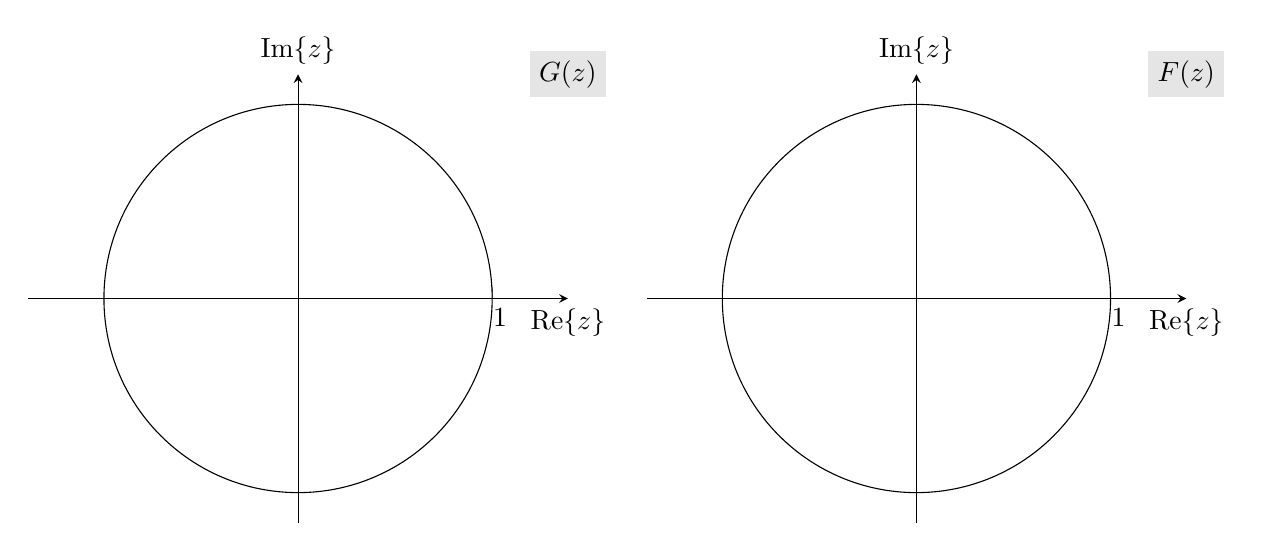
\begin{tikzpicture}
\begin{axis}[
name=plot1,
axis equal,
axis lines*=middle,
enlargelimits = false, clip=true,
xmin=-1.39,
xmax=1.39,
ymin=-1.10,
ymax=1.10,
axis line style={->,>=stealth},
xlabel={$\mathrm{Re}\{z\}$},
ylabel={$\mathrm{Im}\{z\}$},
every axis x label/.style={
at={(ticklabel* cs:1)},
anchor=north,
},
every axis y label/.style={
at={(ticklabel* cs:1)},
anchor=south,
},
xtick=1, ytick=\empty,
xticklabel style={xshift=0.1cm},
every outer y axis line/.append style={white!15!black},
every y tick label/.append style={font=\color{white!15!black}},
legend style={draw=white!15!black,fill=white,legend cell align=left}]
\draw (axis cs:0,0) circle [black!50, dashed, line width=2pt, radius=1];
\if\SOLUTIONS1
\addplot [\SolutionsColor, line width=1pt,mark=x, only marks, mark size = 3pt]
table[row sep=crcr]{
	-0.4714 -0.4714 \\
	-0.4714 0.4714 \\
};

\addplot [\SolutionsColor, line width=1pt,mark=*, only marks, mark size = 3pt, mark options={fill=white}]
table[row sep=crcr]{
	0.3536 0.3536 \\
	0.3536 -0.3536 \\
};
\fi
\end{axis}

\begin{axis}[
name=plot2,
at= (plot1.east), anchor=west, xshift=1cm,
%at=(plot1.below south east), anchor=above north east,
axis equal,
axis lines*=middle,
enlargelimits = false, clip=true,
xmin=-1.39,
xmax=1.39,
ymin=-1.10,
ymax=1.10,
axis line style={->,>=stealth},
xlabel={$\mathrm{Re}\{z\}$},
ylabel={$\mathrm{Im}\{z\}$},
every axis x label/.style={
	at={(ticklabel* cs:1)},
	anchor=north,
},
every axis y label/.style={
	at={(ticklabel* cs:1)},
	anchor=south,
},
xtick=1, ytick=\empty,
xticklabel style={xshift=0.1cm},
every outer y axis line/.append style={white!15!black},
every y tick label/.append style={font=\color{white!15!black}},
legend style={draw=white!15!black,fill=white,legend cell align=left}]
\draw (axis cs:0,0) circle [black!50, dashed, line width=2pt, radius=1];
\if\SOLUTIONS1
  \addplot [\SolutionsColor, line width=1pt,mark=x, only marks, mark size = 3pt]
  table[row sep=crcr]{
		0 	0 \\
  };

  \node[\SolutionsColor, above] at (axis cs: 0.15, 0) {$\times 4$};
  \addplot [\SolutionsColor, line width=1pt,mark=*, only marks, mark size = 3pt, mark options={fill=white}]
  table[row sep=crcr]{
		0.3536 0.3536 \\
		0.3536 -0.3536 \\
		-0.4714 -0.4714 \\
		-0.4714 0.4714 \\
  };
\fi
\end{axis}

\node[black, fill=black!10] at (plot1.north east) {$G(z)$};
\node[black, fill=black!10] at (plot2.north east) {$F(z)$};
\end{tikzpicture}}
	\caption{Poles and zeros of $G(z)$ (left) and $F(z)$ (right).} \label{fig:Hz-inverses}
\end{figure}
\FloatBarrier

\if\SOLUTIONS1
{\color{\SolutionsColor}
	\begin{align} \nonumber
	H(e^{j\omega})F(e^{j\omega}) &= H_{lin}(e^{j\omega}) \\ \nonumber
	F(e^{j\omega}) &= \frac{H_{lin}(e^{j\omega})}{H(e^{j\omega})} = \frac{1}{H_p(e^{j\omega})} \implies F(z) = H_p^{-1}(z)
	\end{align}
}
\else\vspace{1cm}
\fi
\end{description}

\section*{Problem 3: Negative feedback loop (20 points)}
A linear time-invariant system $F(z)$ with input $x[n]$ and output $y[n]$ is described by the difference equation:
\begin{equation}
	y[n] + 4y[n-2] = x[n] -0.5x[n-1],
\end{equation}
\begin{description}
	\item[(a)] (7 points) Give the transfer function $F(z)$. Is this system causal? Is this system stable? What is the ROC of $F(z)$?
	
	\if\SOLUTIONS1
	{\color{\SolutionsColor}
		From the difference equation, we can see that the system is causal since it's output $y[n]$ only depends on current and previous samples of the input and output.
		
		To compute the $z$-transform we just need to apply the linearity and time delay properties of the $z$-transform:
		\begin{align} \nonumber
			Y(z) + 4Y(z)z^{-2} &= X(z) -0.5X(z)z^{-1} \\
			Y(z)(1 + 4z^{-2}) &= X(z)(1 -0.5z^{-1}) \\ \nonumber
			F(z) \equiv \frac{Y(z)}{X(z)} &= \frac{1 -0.5z^{-1}}{1 + 4z^{-2}} \\ \nonumber
			&= \frac{z(z - 0.5)}{z^2 + 4} = \frac{z(z - 0.5)}{(z -2j)(z + 2j)}
		\end{align}
		Thus, this system has two zeros at $z = 0$ and $z = 2$, and two poles at $z = \pm 2j$. As the poles are located outside the unit circle, this system is not stable. The ROC of a causal system is the exterior of a circle whose radius is the outermost poles. Thus, $\mathrm{ROC} = \{|z| > 2\}$.
	}	
	\else\vspace{7cm}
	\fi

\end{description}
\noindent Suppose that $F(z)$ is interconnected in a negative-feedback arrangement with a causal, linear time-invariant system $G(z)$, as shown in Fig.~\ref{fig:feedback-loop}.

\begin{figure}[!h]
	\centering
	\resizebox{0.5\textwidth}{!}{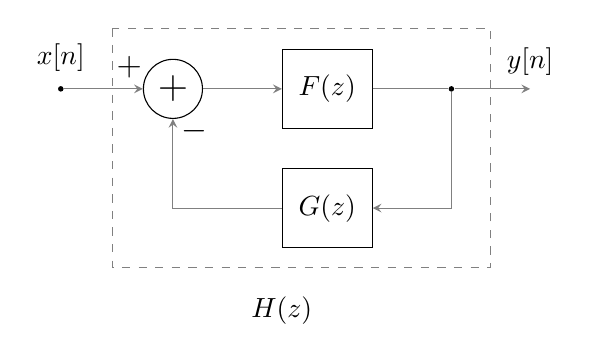
\begin{tikzpicture}[->, >=stealth, shorten >= 0pt, draw=black!50, node distance=3.2cm, font=\sffamily]
    \tikzstyle{node}=[circle,fill=black,minimum size=2pt,inner sep=0pt]
    \tikzstyle{block}=[draw=black,rectangle,fill=none,minimum size=1cm, inner sep=2pt]
    \tikzstyle{add}=[draw=black,circle,fill=none,minimum size=0.75cm, inner sep=2pt]

	\node[node] (xc) {};    
	\node[add, right=1cm of xc, align=center] (S) {\Large $+$};
    \node[block, right=1cm of S, text width = 1cm, align= center] (F) {$F(z)$};
	\node[block, below=0.5cm of F, text width = 1cm, align= center] (G) {$G(z)$};
    \coordinate[right=2cm of F] (yc) {};
    
    \node[node] (mid) at ($(F.east)!0.5!(yc.west)$) {};
    
    \path (xc) edge (S);
    \path (S) edge (F);
    \draw[-] (F) -- (mid);
    \draw (mid) -- (yc);
    \draw (mid) |- (G);
    \draw (G) -| (S);
    
    \node[above = 0.5mm of xc] {$x[n]$};
    \node[above = 0.5mm of yc] {$y[n]$};
    
    \node[left] at ($(S.north west)$) {\large $+$};
    \node[below] at ($(S.south east)$) {\large $-$};

    \draw[dashed] ($(S.north west)+(-0.5cm, 0.5cm)$) rectangle ($(G.south east)+(1.5, -0.25cm)$);
	\node[below] at ($(G.south west) -(0, 0.5cm)$) {$H(z)$};

\end{tikzpicture}}
	\caption{Negative feedback loop.} \label{fig:feedback-loop}
\end{figure}

\begin{description}	

	\item[(b)] (7 points) Derive an expression for the overall system diagram $H(z)$. Your expression should depend on $F(z)$ and $G(z)$ only.
	
	\if\SOLUTIONS1
	{\color{\SolutionsColor}
		\begin{align} \nonumber
			Y(z) &= X(z)F(z) - Y(z)G(z)F(z) \\
			Y(z)(1 + G(z)F(z)) &= X(z)F(z) \\ \nonumber
			H(z) \equiv \frac{Y(z)}{X(z)} &= \frac{F(z)}{1 + G(z)F(z)}
		\end{align}
	}
	\else\vspace{5cm}
	\fi
	
	\item[(c)] (6 points) Find $G(z)$ such that $H(z) = 1$. Is the system $G(z)$ stable?
		
	\noindent Note: By achieving $H(z) = 1$, we're effectively \textit{controlling} the system $F(z)$. That is, we're making $F(z)$ produce whatever output we set it.
	
	\if\SOLUTIONS1
	{\color{\SolutionsColor}
		\begin{align} \nonumber
		z^{-1} &= \frac{F(z)}{1 + G(z)F(z)} \\ \nonumber
		z^{-1}(1 + G(z)F(z)) &= F(z) \\ \nonumber
		G(z) &= 1 - \frac{1}{F(z)} \\ \nonumber
		G(z) &= 1 - \frac{z^2 + 4}{z(z - 0.5)} \\ \nonumber
		G(z) &= -\frac{2(z + 2)}{z(z - 0.5)} \\ \nonumber
		\end{align}
		
		$G(z)$ is causal and it has all its poles inside the unit circle. Thus, it is stable.
	}
	\else\vspace{5cm}
	\fi

\end{description}

%\begin{figure}[!h]
%	\centering
%	\resizebox{0.6\textwidth}{!}{\input{figs/mag-autocorr.tex}}
%	\caption{Sketch of the PSD of the output of $h[n]$ for a white noise input.} \label{fig:mag-resp}
%\end{figure}

\newpage
\section*{Problem 4 (30 points)}

Fig.~\ref{fig:sampling_diagram} shows the block diagram of a digital-signal processing system involving sampling, downconversion, and upsampling. The input to this system $x_c(t)$ is a continuous-time signal, whose Fourier transform is shown in Fig.~\ref{fig:sampling_spectrum}a. This signal is band-limited with maximum frequency given by $\Omega_b$. Suppose that the sampling frequency of the continuous-to-digital converter (C-to-D) is $\Omega_s = 2\Omega_b$. 

\begin{figure}[!h]
	\centering
	\resizebox{\textwidth}{!}{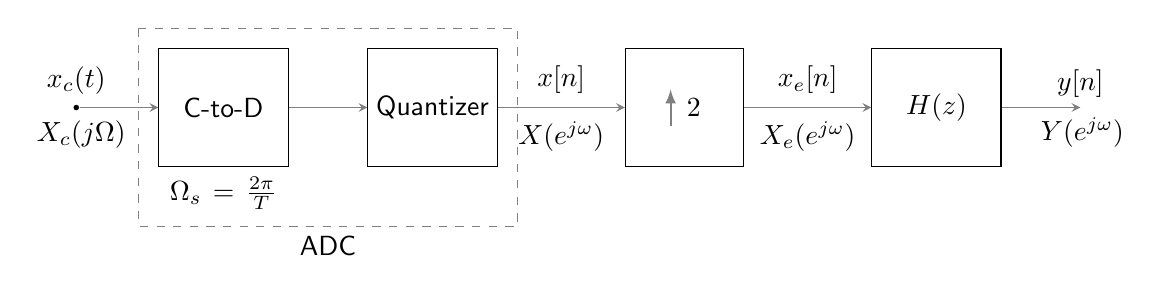
\begin{tikzpicture}[->, >=stealth, shorten >= 0pt, draw=black!50, node distance=3.2cm, font=\sffamily]
    \tikzstyle{node}=[circle,fill=black,minimum size=2pt,inner sep=0pt]
    \tikzstyle{block}=[draw=black,rectangle,fill=none,minimum size=1.5cm, inner sep=2pt]

	\node[node] (xc) {};    
    \node[block, right=1cm of xc, text width = 1.5cm, align= center] (CTD) {C-to-D};
    \node[block, right=1cm of CTD, text width = 1.5cm, align= center] (Q) {Quantizer};
    \node[block, right of=Q, text width = 1cm, align= center] (L) {$~~2$};
    \draw[-latex, shorten >= 15pt, shorten <= 15pt, line width=0.75pt] ($(L.south)-(5pt, 0)$) -- ($(L.north)-(5pt, 0)$) {};
    \node[block, right of=L, text width = 1.5cm, align= center] (H) {$H(z)$};
    \coordinate[right=1cm of H] (yc) {};
    
    \path (xc) edge (CTD);
    \path (CTD) edge (Q);
    \path (Q) edge (L);
    \path (L) edge (H);
    \path (H) edge (yc);
    
    \coordinate (mid1) at ($(Q.east)!0.5!(L.west)$);
    \coordinate (mid2) at ($(L.east)!0.5!(H.west)$);
    
    \node[above = 0.5mm of mid1] {$x[n]$};
    \node[below = 0.5mm of mid1] {$X(e^{j\omega})$};
    \node[above = 0.5mm of mid2] {$x_e[n]$};
    \node[below = 0.5mm of mid2] {$X_e(e^{j\omega})$};
    \node[above = 0mm of xc, text width = 1cm, align=center] {$x_c(t)$};
    \node[below = 0mm of xc, text width = 1cm, align=center] {$X_c(j\Omega)$};
    \node[above = 0mm of yc, text width = 1cm, align=center] {$y[n]$};
    \node[below = 0mm of yc, text width = 1cm, align=center] {$Y(e^{j\omega})$};
    \node[align=center, text width=2cm, below] at ($(CTD.south)$) {$\Omega_s = \frac{2\pi}{T}$};
    
    \draw[dashed] ($(CTD.north west)+(-0.25cm, 0.25cm)$) rectangle ($(Q.south east)+(0.25, -0.75cm)$);
    \node[below] at ($(CTD.south west)!0.5!(Q.south east) -(0, 0.75cm)$) {ADC};
\end{tikzpicture}} 
	\caption{Block diagram of system for problem 4.}\label{fig:sampling_diagram}
\end{figure}


After sampling, the discrete-time signal $x[n]$ is \textit{down-converted}, which is realized by the time-domain multiplication with the signal $e^{-j\pi n}$. This results in the down-converted signal $x_d[n]$. 

After down-conversion, the signal $x_d[n]$ is upsampled by a factor of 2. The resulting signal $x_e[n]$ is filtered by an ideal lowpass filter $H(z)$, whose Fourier transform is given by
\begin{equation}
	H(e^{j\omega}) = \begin{cases}
	1, &|\omega| \leq \pi/4, \\
	0, & \pi/4 < |\omega| < \pi
	\end{cases}.
\end{equation}

\begin{description}
\item[(a)] (28 points) Use the graphs below to sketch the Fourier transform of the signals $x[n]$, $x_d[n]$, $x_e[n]$, $x_f[n]$, obtained after each operation along the system block diagram. Be sure to clearly label all your plots, indicating values in the amplitude and frequency whenever appropriate. Sketches must be clearly labeled and unambiguous to receive full credit. 
\end{description}
\begin{figure}[!h]
\centering
	\resizebox{0.87\textwidth}{!}{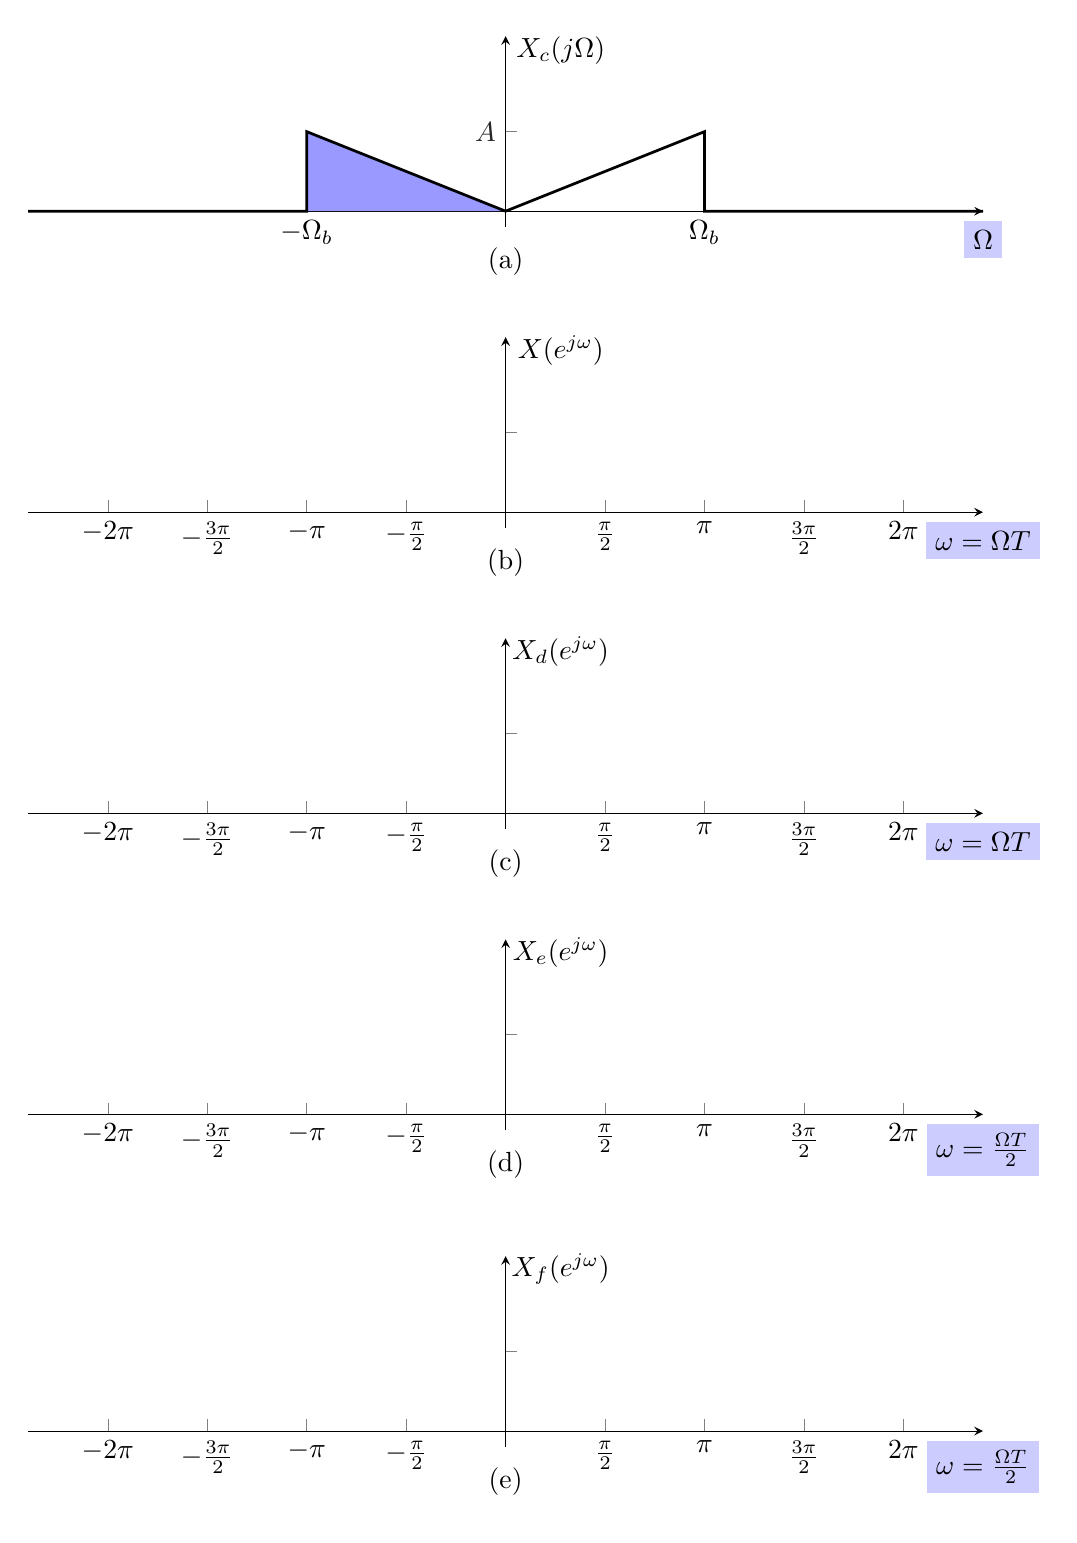
\begin{tikzpicture}
\begin{axis}[
	name=plot1,
	axis lines*=middle,
	enlargelimits = true, clip=true,
	scale only axis,
	width=\textwidth,
	height=0.2\textwidth,
	ymin=0, ymax=2,
	xmin=-4, xmax=4,
	axis line style={->,>=stealth},
	xlabel={ \tikz[baseline]{\node[fill=blue!20,anchor=base] (t1) {$\Omega$};}},
	ylabel={ $X_c(j\Omega)$},
	every axis x label/.style={
		at={(ticklabel* cs:1)},
		anchor=north,
	},
	every axis y label/.style={
		at={(ticklabel* cs:0.8)},
		anchor=south,
		xshift=0.7cm,
	},	
	ytick=1,
	yticklabels={ $A$},
	xtick={-2, 0, 2},
	xticklabels={ $-\Omega_b$,  0, $\Omega_b$}, 
	every outer y axis line/.append style={white!15!black},
	every y tick label/.append style={font=\color{white!15!black}},
	legend style={draw=white!15!black,fill=white,legend cell align=left}]
	\addplot[solid, line width=1pt] coordinates {(0, 0) (2, 1) (2, 0) (7, 0)};
    \addplot[solid, fill=blue!40, line width=1pt] coordinates {(-7, 0) (-2, 0) (-2, 1) (0, 0)};
\end{axis}

\begin{axis}[
	name=plot2,
    at=(plot1.below south east), anchor=above north east, yshift=-0.75cm,
	axis lines*=middle,
	enlargelimits = true,	clip=true,
	scale only axis,
	width=\textwidth,
	height=0.2\textwidth,
	ymin=0, ymax=2,
	xmin=-4, xmax=4,
	axis line style={->,>=stealth},
	xlabel={ \tikz[baseline]{\node[fill=blue!20,anchor=base] (t1) {$\omega = \Omega T$};}},
	ylabel={ $X(e^{j\omega})$},
	every axis x label/.style={
		at={(ticklabel* cs:1)},
		anchor=north,
	},
	every axis y label/.style={
		at={(ticklabel* cs:0.8)},
		anchor=south,
		xshift=0.7cm,
	},	
	ytick=1,
	yticklabels={ },
	xtick={-4, ..., 4},
	xticklabels={$-2\pi$, $-\frac{3\pi}{2}$, $-\pi$, $-\frac{\pi}{2}$, 0, $\frac{\pi}{2}$, $\pi$, $\frac{3\pi}{2}$, $2\pi$}, 
	every outer y axis line/.append style={white!15!black},
	every y tick label/.append style={font=\color{white!15!black}},
	legend style={draw=white!15!black,fill=white,legend cell align=left}]
	
	\if\SOLUTIONS1
		\node at (axis cs: 0.5, 1) {$A/T$};
		\foreach \df in {-8, -4, 0, 4, 8}
		{
			\edef\temp{\noexpand\addplot[solid, line width=1pt] coordinates {(0+\df, 0) (2+\df, 1) (2+\df, 0) (7+\df, 0)};}
			\temp
			\edef\temp{\noexpand\addplot[solid, fill=blue!40, line width=1pt] coordinates {(-7+\df, 0) (-2+\df, 0) (-2+\df, 1) (0+\df, 0)};}
			\temp
		}
 	\fi
\end{axis}

\begin{axis}[
name=plot3,
at=(plot2.below south east), anchor=above north east, yshift=-0.75cm,
axis lines*=middle,
enlargelimits = true, clip=true,
scale only axis,
width=\textwidth,
height=0.2\textwidth,
ymin=0, ymax=2,
xmin=-4, xmax=4,
axis line style={->,>=stealth},
xlabel={ \tikz[baseline]{\node[fill=blue!20,anchor=base] (t1) {$\omega = \Omega T$};}},
ylabel={ $X_d(e^{j\omega})$},
every axis x label/.style={
	at={(ticklabel* cs:1)},
	anchor=north,
},
every axis y label/.style={
	at={(ticklabel* cs:0.8)},
	anchor=south,
	xshift=0.7cm,
},	
ytick=1,
yticklabels={ },
xtick={-4, ..., 4},
xticklabels={$-2\pi$, $-\frac{3\pi}{2}$, $-\pi$, $-\frac{\pi}{2}$, 0, $\frac{\pi}{2}$, $\pi$, $\frac{3\pi}{2}$, $2\pi$},  
every outer y axis line/.append style={white!15!black},
every y tick label/.append style={font=\color{white!15!black}},
legend style={draw=white!15!black,fill=white,legend cell align=left}]

\if\SOLUTIONS1
\node at (axis cs: 0.5, 1) {$A/T$};
\foreach \df in {-10, -6, -2, 2, 6, 10}
{
	\edef\temp{\noexpand\addplot[solid, line width=1pt] coordinates {(0+\df, 0) (2+\df, 1) (2+\df, 0) (7+\df, 0)};}
	\temp
	\edef\temp{\noexpand\addplot[solid, fill=blue!40, line width=1pt] coordinates {(-7+\df, 0) (-2+\df, 0) (-2+\df, 1) (0+\df, 0)};}
	\temp
}
\fi
\end{axis}

\begin{axis}[
name=plot4,
at=(plot3.below south east), anchor=above north east, yshift=-0.75cm,
axis lines*=middle,
enlargelimits = true, clip=true,
scale only axis,
width=\textwidth,
height=0.2\textwidth,
ymin=0, ymax=2,
xmin=-4, xmax=4,
axis line style={->,>=stealth},
xlabel={ \tikz[baseline]{\node[fill=blue!20,anchor=base] (t1) {$\omega = \frac{\Omega T}{2}$};}},
ylabel={ $X_e(e^{j\omega})$},
every axis x label/.style={
	at={(ticklabel* cs:1)},
	anchor=north,
},
every axis y label/.style={
	at={(ticklabel* cs:0.8)},
	anchor=south,
	xshift=0.7cm,
},	
ytick=1,
yticklabels={ },
xtick={-4, ..., 4},
xticklabels={$-2\pi$, $-\frac{3\pi}{2}$, $-\pi$, $-\frac{\pi}{2}$, 0, $\frac{\pi}{2}$, $\pi$, $\frac{3\pi}{2}$, $2\pi$}, 
every outer y axis line/.append style={white!15!black},
every y tick label/.append style={font=\color{white!15!black}},
legend style={draw=white!15!black,fill=white,legend cell align=left}]

\if\SOLUTIONS1
\node at (axis cs: 0.5, 1) {$A/T$};
\foreach \df in {-8,-6,..., 8}
{
	\edef\temp{\noexpand\addplot[solid, line width=1pt] coordinates {(-1+\df, 0) (0+\df, 1) (0+\df, 0) (\df, 0)};}
	\temp
	\edef\temp{\noexpand\addplot[solid, fill=blue!40, line width=1pt] coordinates {(\df, 0) (\df, 1) (1+\df, 0) (\df, 0)};}
	\temp
}
\fi
\end{axis}

\begin{axis}[
name=plot5,
at=(plot4.below south east), anchor=above north east, yshift=-0.75cm,
axis lines*=middle,
enlargelimits = true, clip=true,
scale only axis,
width=\textwidth,
height=0.2\textwidth,
ymin=0, ymax=2,
xmin=-4, xmax=4,
axis line style={->,>=stealth},
xlabel={ \tikz[baseline]{\node[fill=blue!20,anchor=base] (t1) {$\omega = \frac{\Omega T}{2}$};}},
ylabel={ $X_f(e^{j\omega})$},
every axis x label/.style={
	at={(ticklabel* cs:1)},
	anchor=north,
},
every axis y label/.style={
	at={(ticklabel* cs:0.8)},
	anchor=south,
	xshift=0.7cm,
},	
ytick=1,
yticklabels={},
xtick={-4, ..., 4},
xticklabels={$-2\pi$, $-\frac{3\pi}{2}$, $-\pi$, $-\frac{\pi}{2}$, 0, $\frac{\pi}{2}$, $\pi$, $\frac{3\pi}{2}$, $2\pi$}, 
every outer y axis line/.append style={white!15!black},
every y tick label/.append style={font=\color{white!15!black}},
legend style={draw=white!15!black,fill=white,legend cell align=left}]

\if\SOLUTIONS1
\node at (axis cs: 0.5, 1) {$A/T$};
\foreach \df in {-8,-4,..., 8}
{
	\edef\temp{\noexpand\addplot[solid, line width=1pt] coordinates {(-4+\df, 0) (-0.5+\df, 0) (-0.5+\df, 0.5) (\df, 1) (\df, 0) (-0.5+\df, 0)};}
	\temp
	\edef\temp{\noexpand\addplot[solid, fill=blue!40, line width=1pt] coordinates {(\df, 0) (\df, 1) (0.5+\df, 0.5) (0.5+\df, 0) (\df, 0)};}
	\temp
}
\fi
\end{axis}

\node[below, inner sep=0.25cm] at (plot1.south) {(a)};
\node[below, inner sep=0.25cm] at (plot2.south) {(b)};
\node[below, inner sep=0.25cm] at (plot3.south) {(c)};
\node[below, inner sep=0.25cm] at (plot4.south) {(d)};
\node[below, inner sep=0.25cm] at (plot5.south) {(e)};


\end{tikzpicture}
}
    \caption{Spectrum plots for Problem 4.} \label{fig:sampling_spectrum}
\end{figure}


\begin{description}
\item[(b)]  (2 points) Suppose that we would like to downsample the output signal $x_f[n]$. What is the largest downsampling rate that we could use to downsample $x_f[n]$ and still avoid aliasing? Justify. \\
\if\SOLUTIONS1
{\color{\SolutionsColor}
The largest downsampling factor is 4, since the ideal lowpass filter cutoff frequency is $\pi/4$.
}
\else\vspace{1cm}
\fi

\end{description}
\newpage
%\item[(b)] (6 points) Suppose that $\Omega_c = 8\pi$ rad/s and $\Omega_b = \pi$ rad/s. Draw the spectrum of $x[n]$ when $x_c(t)$ is sampled with sampling frequency $\Omega_s = 2\pi$ rad/s  (much smaller than the Nyquist rate). 
%
%\begin{figure}[!h]
%\centering
%	\resizebox{\textwidth}{!}{\begin{tikzpicture}
\begin{axis}[
	name=plot1,
	axis lines*=middle,
	enlargelimits = false, clip=true,
	scale only axis,
	width=\textwidth,
	height=0.2\textwidth,
	ymin=0, ymax=1.5,
	xmin=-6, xmax=6,
	axis line style={->,>=stealth, shorten >= -0.7cm},
	xlabel={ \tikz[baseline]{\node[fill=blue!20,anchor=base] (t1) {$\omega$};}},
	ylabel={ $X(e^{j\omega})$},
	every axis x label/.style={
		at={(ticklabel* cs:1)},
		anchor=north,
        xshift=0.6cm,
	},
	every axis y label/.style={
		at={(ticklabel* cs:1)},
		anchor=south,
		xshift=0.7cm,
	},	
	ytick=1,
    yticklabels={$A/T$},
	xtick={-6,-4,...,6},
	xticklabels={$-3\pi$, $-2\pi$,  $-\pi$, $0$, $\pi$, $2\pi$, $3\pi$}, 
    xmajorgrids,
	every outer y axis line/.append style={white!15!black},
	every y tick label/.append style={font=\color{white!15!black}},
	legend style={draw=white!15!black,fill=white,legend cell align=left}]
    \if\SOLUTIONS1
      \ifdefined\SolD
        \def\fs{4}
        \foreach \k in {-1, 0, 1} {
          \addplot[solid, line width=1pt] coordinates {(0-\k*\fs-\fs/2, 0) (0-\k*\fs-\fs/2, 1) (2-\k*\fs-\fs/2, 0)};
          \addplot[solid, fill=blue!40, line width=1pt] coordinates {(-2-\k*\fs+\fs/2, 0) (0-\k*\fs+\fs/2, 1) (0-\k*\fs+\fs/2, 0)};
          }
      \else
      	\def\fs{4}
        \foreach \k in {-1, 0, 1} {
          \addplot[solid, line width=1pt] coordinates {(0-\k*\fs, 1) (2-\k*\fs, 0)};
          \addplot[solid, fill=blue!40, line width=1pt] coordinates {(-2-\k*\fs, 0) (0-\k*\fs, 1) (0-\k*\fs, 0)};
      }
      \fi
   \fi
\end{axis}
\end{tikzpicture}}\label{fig:bp_spectrum_sol1}
%\end{figure}
%\if\SOLUTIONS0\vspace{5cm}
%\fi
%
%\item[(c)] (7 points) In part (b) you saw that there is no spectrum overlap, even though $x_c(t)$ was sampled below the Nyquist rate. Is that always possible? Give conditions on the sampling frequency $\Omega_s$ in terms of $\Omega_c$ and $\Omega_b$ so that: (i) the spectrum is centered around $\omega = 0$ as in Figure~\ref{fig:bp_spectrum1}b, \underline{and} (ii) such that there is no spectrum overlap. 
%
%\textit{Hint:} The spectrum replicas occur according to the sampling equation:
%\begin{equation}
%X(e^{j\Omega T}) = \frac{1}{T}\sum_{k=-\infty}^\infty X_c(j(\Omega-k\Omega_s))
%\end{equation}
%
%\if\SOLUTIONS1
%{\color{\SolutionsColor}
%Staring with the sampling equation we have the following conditions:
%
%(i) In order to bring the signal down to baseband:
%\begin{align*}
%0 - k\Omega_s = \Omega_c \implies \Omega_c = -k\Omega_s
%\end{align*}
%for some negative integer $k$.
%
%(ii) The ($-k-1$)th spectrum replica must fall at least at $-2\Omega_b$ in order to avoid spectrum overlap. Therefore, 
%\begin{align*} \nonumber
%-2\Omega_b - (k-1)\Omega_s &\geq \Omega_c \\ \nonumber
%-2\Omega_b - (k-1)\Omega_s &\geq -k\Omega_s \tag{since $\Omega_c = -k\Omega_s$} \\
%\Omega_s &\geq 2\Omega_b
%\end{align*}
%}
%\else\vspace{10cm}
%\fi
%
%
%\item[(d)] (5 points) Repeat part (b), but now assume that $\Omega_c = 7\pi$ rad/s and $\Omega_b = \pi$ rad/s. Sampling is still performed with sampling frequency $\Omega_s = 2\pi$ rad/s. 
%
%\textit{Note:} Although there isn't spectrum overlap in this case either, further processing would be necessary to center the spectrum around $\omega = 0$, as in Figure~\ref{fig:bp_spectrum1}b.
%
%\begin{figure}[!h]
%\centering
%	\def\SolD{1}
%	\resizebox{\textwidth}{!}{\begin{tikzpicture}
\begin{axis}[
	name=plot1,
	axis lines*=middle,
	enlargelimits = false, clip=true,
	scale only axis,
	width=\textwidth,
	height=0.2\textwidth,
	ymin=0, ymax=1.5,
	xmin=-6, xmax=6,
	axis line style={->,>=stealth, shorten >= -0.7cm},
	xlabel={ \tikz[baseline]{\node[fill=blue!20,anchor=base] (t1) {$\omega$};}},
	ylabel={ $X(e^{j\omega})$},
	every axis x label/.style={
		at={(ticklabel* cs:1)},
		anchor=north,
        xshift=0.6cm,
	},
	every axis y label/.style={
		at={(ticklabel* cs:1)},
		anchor=south,
		xshift=0.7cm,
	},	
	ytick=1,
    yticklabels={$A/T$},
	xtick={-6,-4,...,6},
	xticklabels={$-3\pi$, $-2\pi$,  $-\pi$, $0$, $\pi$, $2\pi$, $3\pi$}, 
    xmajorgrids,
	every outer y axis line/.append style={white!15!black},
	every y tick label/.append style={font=\color{white!15!black}},
	legend style={draw=white!15!black,fill=white,legend cell align=left}]
    \if\SOLUTIONS1
      \ifdefined\SolD
        \def\fs{4}
        \foreach \k in {-1, 0, 1} {
          \addplot[solid, line width=1pt] coordinates {(0-\k*\fs-\fs/2, 0) (0-\k*\fs-\fs/2, 1) (2-\k*\fs-\fs/2, 0)};
          \addplot[solid, fill=blue!40, line width=1pt] coordinates {(-2-\k*\fs+\fs/2, 0) (0-\k*\fs+\fs/2, 1) (0-\k*\fs+\fs/2, 0)};
          }
      \else
      	\def\fs{4}
        \foreach \k in {-1, 0, 1} {
          \addplot[solid, line width=1pt] coordinates {(0-\k*\fs, 1) (2-\k*\fs, 0)};
          \addplot[solid, fill=blue!40, line width=1pt] coordinates {(-2-\k*\fs, 0) (0-\k*\fs, 1) (0-\k*\fs, 0)};
      }
      \fi
   \fi
\end{axis}
\end{tikzpicture}} \label{fig:bp_spectrum_sol1}
%\end{figure}
%\if\SOLUTIONS0\vspace{5cm}
%\fi
%
%\end{description}
%
%\newpage
%\section*{Problem 4: (20 points)}
%The diagram of Figure~\ref{fig:sampling_diagram} represents the initial DSP of a high-speed application. Since fast ADCs are expensive, the design engineers decided to perform Nyquist-rate sampling and upsample the signal immediately after the ADC, as illustrated in Figure~\ref{fig:sampling_diagram}. The lowpass filter $H(z)$ after upsampling is used to eliminate unwanted spectrum replicas of the signal and of quantization noise. The additive white  noise introduced by the quantizer has average power $\sigma_Q^2$.
%
%
%
%\begin{description}
%\item[(a)] (8 points) The plot below shows the spectrum $X(e^{j\omega})$ with signal (triangular shape) and quantization noise (dashed red line) components. Use the empty graphs below to sketch $X_e(e^{j\omega})$ and $Y(e^{j\omega})$. In your plots, draw both the signal and noise components. Assume that $H(z)$ is the ideal lowpass filter with cutoff frequency $\pm\pi/2$ and \underline{unit gain}.
%
%\textit{Hint:} consider signal and noise separately.
% 
%\FloatBarrier
%\begin{figure}[!h]
%\centering
%	\resizebox{0.9\textwidth}{!}{% \fs and \fmax must be defined before calling this picture.
\def\fs{5}
\def\fmax{2.5}
\begin{tikzpicture}
\begin{axis}[
	name=plot2,
	%at=(plot1.below south east), anchor=above north east,
	axis lines*=middle,
	enlargelimits = true,
	clip=true,
	scale only axis,
	width=\textwidth,
	height=0.2\textwidth,
	ymin=0,
	ymax=3,
	xmin=-\fs-1,
	xmax=\fs+1,
	axis line style={->,>=stealth},
	xlabel={\small \tikz[baseline]{\node[fill=blue!20,anchor=base] (t1) {$\omega = \Omega T$};}},
	ylabel={\small $X(e^{j\omega})$},
	every axis x label/.style={
		at={(ticklabel* cs:1)},
		anchor=north,
	},
	every axis y label/.style={
		at={(ticklabel* cs:0.8)},
		anchor=south,
		xshift=0.6cm,
	},
	xtick=\empty,
	ytick=2,
	yticklabels={\small $\frac{1}{T}$},
	yticklabel style={yshift=0.1cm},
	xtick={-\fs, -2.5, 0, 2.5, \fs},
	xticklabels={\small $-2\pi$, \small $-\pi$, \small 0, \small $\pi$, \small $2\pi$}, 
	every outer y axis line/.append style={white!15!black},
	every y tick label/.append style={font=\color{white!15!black}},
	legend style={draw=white!15!black,fill=white,legend cell align=left}]
	\addplot[solid, line width=1pt] coordinates {(0, 2) (2.5, 0) (0, 0)};
	\addplot[solid, line width=1pt, fill=blue!50] coordinates {(0, 2) (-2.5, 0) (0, 0)};
	\addplot[solid, line width=1pt] coordinates {(\fs, 2) (\fs+2.5, 0) (\fs, 0)};
	\addplot[solid, line width=1pt, fill=blue!50] coordinates {(\fs, 2) (\fs-2.5, 0) (\fs, 0)};
	\addplot[solid, line width=1pt] coordinates {(-\fs, 2) (-\fs+2.5, 0) (-\fs, 0)};
	\addplot[solid, line width=1pt, fill=blue!50] coordinates {(-\fs, 2) (-\fs-2.5, 0) (-\fs, 0)};
	\addplot[solid, line width=1pt] coordinates {(-2*\fs, 2) (-2*\fs+2.5, 0) (-2*\fs, 0)};
	\addplot[solid, line width=1pt, fill=blue!50] coordinates {(-2*\fs, 2) (-2*\fs-2.5, 0) (-2*\fs, 0)};]
	\addplot[solid, line width=1pt] coordinates {(2*\fs, 2) (2*\fs+2.5, 0) (2*\fs, 0)};
	\addplot[solid, line width=1pt, fill=blue!50] coordinates {(2*\fs, 2) (2*\fs-2.5, 0) (2*\fs, 0)};
    \addplot[red2, line width=1.5pt, dashed] coordinates {(-3*\fs, 0) (-3*\fs, 0.7) (3*\fs, 0.7) (3*\fs, 0)} node[pos=0.57, black, pin={[pin edge={red, solid, thick}]30:{$\sigma_Q^2$}}, inner sep=0pt] {};
\end{axis}

\def\fsM{2.5}
\def\fmaxM{1.25} % 
\def\BWM{1.25} % WN * T_d = WN * 2 * T = 2 * (BW)
\begin{axis}[
	name=plot3,
	at=(plot2.below south east), anchor=above north east,
	axis lines*=middle,
	enlargelimits = true,
	clip=true,
	scale only axis,
	width=\textwidth,
	height=0.2\textwidth,
	ymin=0,
	ymax=3,
	xmin=-\fs-1,
	xmax=\fs+1,
	axis line style={->,>=stealth},
	xlabel={\small \tikz[baseline]{\node[fill=blue!20,anchor=base] (t1) {$\omega = \frac{\Omega T}{2}$};}},
	ylabel={\small $X_e(e^{j\omega}) = X(e^{j\omega L})$},
	every axis x label/.style={
		at={(ticklabel* cs:1)},
		%xshift=0.2cm,
		anchor=north,
	},
	every axis y label/.style={
		at={(ticklabel* cs:0.8)},
		anchor=south,
		xshift=1.5cm,
	},
	xtick=\empty,
	ytick=2,
	yticklabels={\small $\frac{1}{T}$},
	xtick={-5, -3.75, ..., 5},
	xticklabels={\small $-2\pi$, \small $-\frac{3\pi}{2}$, \small $-\pi$, \small $-\frac{\pi}{2}$, 0, \small $\frac{\pi}{2}$, \small $\pi$, \small $\frac{3\pi}{2}$, \small $2\pi$}, 
	every outer y axis line/.append style={white!15!black},
	every y tick label/.append style={font=\color{white!15!black}},
	legend style={draw=white!15!black,fill=white,legend cell align=left}]
    \if\SOLUTIONS1
	\addplot[solid, line width=1pt] coordinates {(0, 2) (\BWM, 0) (0, 0)};
	\addplot[solid, line width=1pt, fill=blue!50] coordinates {(0, 2) (-\BWM, 0) (0, 0)};
	\addplot[solid, line width=1pt] coordinates {(\fsM, 2) (\fsM+\BWM, 0) (\fsM, 0)};
	\addplot[solid, line width=1pt, fill=blue!50] coordinates {(\fsM, 2) (\fsM-\BWM, 0) (\fsM, 0)};
	\addplot[solid, line width=1pt] coordinates {(-\fsM, 2) (-\fsM+\BWM, 0) (-\fsM, 0)};
	\addplot[solid, line width=1pt, fill=blue!50] coordinates {(-\fsM, 2) (-\fsM-\BWM, 0) (-\fsM, 0)};
	\addplot[solid, line width=1pt] coordinates {(-2*\fsM, 2) (-2*\fsM+\BWM, 0) (-2*\fsM, 0)};
	\addplot[solid, line width=1pt, fill=blue!50] coordinates {(-2*\fsM, 2) (-2*\fsM-\BWM, 0) (-2*\fsM, 0)};]
	\addplot[solid, line width=1pt] coordinates {(2*\fsM, 2) (2*\fsM+\BWM, 0) (2*\fsM, 0)};
	\addplot[solid, line width=1pt, fill=blue!50] coordinates {(2*\fsM, 2) (2*\fsM-\BWM, 0) (2*\fsM, 0)};
	\node[scale=1, fill=black!20] at (axis cs: 5, 2) {Upsampled by 2};
    \addplot[red2, line width=1.5pt, dashed] coordinates {(-3*\fs, 0) (-3*\fs, 0.7) (3*\fs, 0.7) (3*\fs, 0)} node[pos=0.45, black, pin={[pin edge={red, solid, thick}]30:{$\sigma_Q^2$}}, inner sep=0pt] {};
    \fi
\end{axis}

\def\fbw{1.25}
\begin{axis}[
	name=plot4,
	at=(plot3.below south east), anchor=above north east,
	axis lines*=middle,
	enlargelimits = true, clip=true,
	scale only axis,
	width=\textwidth,
	height=0.2\textwidth,
	ymin=0,
	ymax=3,
	xmin=-\fs-1,
	xmax=\fs+1,
	axis line style={->,>=stealth},
	xlabel={\small \tikz[baseline]{\node[fill=blue!20,anchor=base] (t1) {$\omega = \frac{\Omega T}{2}$};}},
	ylabel={\small $Y(e^{j\omega})$},
	every axis x label/.style={
		at={(ticklabel* cs:1)},
		%xshift=0.2cm,
		anchor=north,
	},
	every axis y label/.style={
		at={(ticklabel* cs:0.8)},
		anchor=south,
		xshift=0.6cm,
	},
	xtick=\empty,
    ytick=2,
    yticklabels={\small $\frac{1}{T}$},
	yticklabel style={yshift=0.2cm},
	xtick={-5, -3.75, ..., 5},
	xticklabels={\small $-2\pi$, \small $-\frac{3\pi}{2}$, \small $-\pi$, \small $-\frac{\pi}{2}$, 0, \small $\frac{\pi}{2}$, \small $\pi$, \small $\frac{3\pi}{2}$, \small $2\pi$}, 
	every outer y axis line/.append style={white!15!black},
	every y tick label/.append style={font=\color{white!15!black}},
	legend style={draw=white!15!black,fill=white,legend cell align=left}]
    \if\SOLUTIONS1
	\addplot[solid, line width=1pt] coordinates {(0, 2) (\BWM, 0) (0, 0)};
	\addplot[solid, line width=1pt, fill=blue!50] coordinates {(0, 2) (-\BWM, 0) (0, 0)};
	\addplot[solid, line width=1pt] coordinates {(-2*\fsM, 2) (-2*\fsM+\BWM, 0) (-2*\fsM, 0)};
	\addplot[solid, line width=1pt, fill=blue!50] coordinates {(-2*\fsM, 2) (-2*\fsM-\BWM, 0) (-2*\fsM, 0)};]
	\addplot[solid, line width=1pt] coordinates {(2*\fsM, 2) (2*\fsM+\BWM, 0) (2*\fsM, 0)};
	\addplot[solid, line width=1pt, fill=blue!50] coordinates {(2*\fsM, 2) (2*\fsM-\BWM, 0) (2*\fsM, 0)};
    \addplot[red2, line width=1.5pt, dashed] coordinates {(-2*\fsM-\BWM, 0) (-2*\fsM-\BWM, 0.75) (-2*\fsM+\BWM, 0.75) (-2*\fsM+\BWM, 0) (-\BWM, 0) (-\BWM, 0.75) (\BWM, 0.75) (\BWM, 0) (2*\fsM-\BWM, 0) (2*\fsM-\BWM, 0.75) (2*\fsM-\BWM, 0.75) (2*\fsM+\BWM, 0.75) (2*\fsM+\BWM, 0)} node[pos=0.57, black, pin={[pin edge={red, solid, thick}]30:{$\sigma_Q^2$}}, inner sep=0pt] {};
    \fi
\end{axis}

\end{tikzpicture}
} \label{fig:spectrum_upsample}
%\end{figure}
%\FloatBarrier
%
%\item[(b)] (6 points) Now assume that $H(z)$ is the first-order lowpass filter given by
%\begin{equation}
%H(z) = \frac{1 + cz^{-1}}{1 - cz^{-1}}, \qquad 0 < c < 1.
%\end{equation}
%
%Assume that this filter is implemented using the transposed direct form II with signal values and filter coefficients scaled as Q15 integers. The result of multiplications is quantized to 16-bits (15 bits plus sign) \underline{immediately after} the multiplications and \underline{before} any additions are done. Draw the signal flow graph diagram of this system. In your drawing include noise sources representing the quantization of the multiplications. Label each noise source with average power $\sigma_{15}^2$. You may combine noise sources whenever possible. In addition, circle \underline{all nodes} in which overflow may happen.
%
%\textit{Note:} You do not need to include noise sources in multiplications by 1.
%
%\if\SOLUTIONS1
%{\color{\SolutionsColor}
%Overflow may happen in any node in which additions are performed. Multiplications do not overflow. 
%
%The noise sources were combined into one with average power $2\sigma_{15}^2$. Note that since $b_0 = 1$, in this case, then this multiplication is not performed and therefore we should not include a noise source for it.
%
%\FloatBarrier
%\begin{figure}[h!]
%\centering
%	\def\SolD{1}
%	\resizebox{0.5\textwidth}{!}{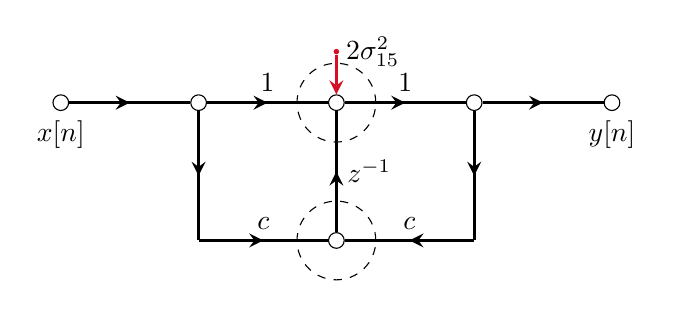
\begin{tikzpicture}[node distance=1.75cm]
\tikzstyle{node}=[circle,fill=red2,minimum size=2pt,inner sep=0pt]
%Place the nodes
\node[terminal={below}{$x[n]$}] (x) at (0,0) {};
\node[terminal={below}{}, right of=x] (00) {};
\node[terminal={below}{}, right of= 00] (01) {};
\node[terminal={below}{}, right of=01] (02) {};
\node[terminal={below}{$y[n]$}, right of=02] (y) {};

\foreach \j in {1} {
	\pgfmathtruncatemacro{\jn}{(\j-1)}%
	\coordinate[below of=\jn0] (\j0) {};
	\node[terminal={below}{}, below of=\jn1] (\j1) {};
	\coordinate[below of=\jn2] (\j2) {};
}

%
\draw[zpath={right}] (11) to (01);

%
\draw[amark] (00) to (10);
\draw[amark] (02) to (12);


%
\draw[amark={$1$}{above}] (00) to (01);
\draw[amark={$c$}{above}] (10) to (11);

%
\draw[amark={$1$}{above}] (01) to (02);
\draw[amark={$c$}{above}] (12) to (11);


\draw[amark] (x) to (00);
\draw[amark] (02) to (y);

\draw[dashed] (01) circle[radius=0.5cm];
\draw[dashed] (11) circle[radius=0.5cm];

\node[node, above=0.5cm of 01] (E) {}; \node[right] at (E) {$2\sigma_{15}^2$};
\draw[->, >=stealth, red2, \thickness] (E) to (01);

\end{tikzpicture}}
%\end{figure}
%\FloatBarrier
%}
%\else\vspace{7cm}
%\fi
%
%\item{(c)} (6 points) Write an equation for the PSD of the total noise at the output of $H(z)$. The total noise includes quantization noise from the quantizer and roundoff noise from your filter implementation in part (b). Write your answer in terms of $\sigma_{15}^2$, $\sigma_{Q}^2$, and $c$.
%
%\if\SOLUTIONS1
%{\color{\SolutionsColor}
%Using superposition, we see that the quantization noise is filtered by $H(z)$, while the roundoff noise is filtered only by the poles of $H(z)$, which we'll denoted by $\frac{1}{A(z)}$. Therefore,
%
%\begin{align*}
%\Phi_{ff}(e^{j\omega}) &= \sigma_Q^2|H(e^{j\omega})|^2 + 2\sigma_{15}^2\frac{1}{|A(e^{j\omega})|} \\
%&= \sigma_Q^2|H(e^{j\omega})|^2 + 2\sigma_{15}^2\frac{1}{|A(e^{j\omega})|} \\
%& = \frac{\sigma_Q^2(1 + c^2 + 2c\cos\omega) + 2\sigma_{15}^2}{1 + c^2 - 2c\cos\omega}
%\end{align*}
%
%}
%\else\vspace{5cm}
%\fi
%\end{description}


\end{document}
